\documentclass[a4paper,10pt]{article}
\usepackage[utf8]{inputenc}
\usepackage[colorlinks,plainpages=false]{hyperref}

\setlength\parindent{0pt}
\usepackage[english]{babel}
\usepackage[dvinames]{xcolor}
\usepackage[compact,small]{titlesec}
\usepackage{booktabs}
\usepackage{multirow}
\usepackage{amsfonts,amsmath,amssymb}
\usepackage{marginnote}
\usepackage[top=1.8cm, bottom=1.8cm, outer=1.8cm, inner=1.8cm, heightrounded, marginparwidth=2.5cm, marginparsep=0.5cm]{geometry}
\usepackage{enumitem}
\setlist{noitemsep,parsep=2pt}
\newcommand{\highlight}[1]{\textcolor{kuleuven}{#1}}
\usepackage{pythonhighlight}
\usepackage{cleveref}
\usepackage{graphicx}
\graphicspath{{Pictures/}}
\usepackage{algorithmic}
\usepackage{tabularx}
\usepackage{bm}
\usepackage{subcaption}
\usepackage{array}


\newcommand{\nextyear}{\advance\year by 1 \the\year\advance\year by -1}
\newcommand{\thisyear}{\the\year}
\newcommand{\deadlineGroup}{November 27, \thisyear{} at 16:00 CET}
\newcommand{\deadlineCode}{December 18, \thisyear{} at 16:00 CET}
\newcommand{\deadlineReport}{January 4, \nextyear{} at 16:00 CET}

\newcommand{\ReplaceMe}[1]{{\color{blue}#1}}
\newcommand{\RemoveMe}[1]{{\color{purple}#1}}

\setlength{\parskip}{5pt}

%opening
\title{Artificial Neural Networks: Exercise session 4}
\author{Stijn Staring (r0620003)}

\begin{document}
\fontfamily{ppl}
\selectfont{}

\maketitle


\section{Restricted Boltzmann Machines}
The Boltzmann machine is a parametrized generative model representing a probability distribution. It is a neural network that belong to Energy based models. A Boltzmann Machine consist out of a layer of visible units $ \bm{v} $ and hidden units $ \bm{h} $. The standard type of BM uses binary-valued hidden and visible units. The difference between a Restricted Boltzmann Machine and a conventional  Boltzmann Machine, is that the units of one layer are not connected with each other. Because of this restriction, the partition function in the joint probability seen in Eq. \ref{} becomes tractable. Training an RBM means adjusting the RBM weight values and  biases such that the probability distribution Eq. \ref{eq:1b} fits the training data as well as possible. 


 An RBM trains in an unsupervised manner. 
\begin{subequations}
	\begin{equation}
		E(\bm{v},\bm{h}) = -\bm{v}^T\bm{W}\bm{h} - \bm{b}^T\bm{v}-\bm{a}^T\bm{h},
	\end{equation}
	\begin{equation}
		P(\bm{v},\bm{h}) = \frac{1}{Z}e^{-E(\bm{v},\bm{h})}    .
	\end{equation}
	\label{eq:1}
\end{subequations}

Eq. \ref{eq:1}

Training is done --> making updates by calculating gradient with the log likelihood. 



\begin{table}[h]
	\begin{minipage}[t]{.5\linewidth}
		\centering
			\begin{tabular}{@{}l|ccc}
				\firsthline
				\textbf{Learning rate}/\textbf{Iterations}	&  5 & 10 & 20 \\ \midrule
				0,005&	141	&134&	127,41	\\ \hline
				0,01&	166&	147,66&	125,55\\ \hline
				0,05 &	141,15&	134,35&	127,41\\ \hline
				0,1 &	134,46&	130,24&	130,81\\\bottomrule
			\end{tabular}		
	\end{minipage}
	\begin{minipage}[t]{.5\linewidth}
		\centering
		\begin{tabular}{@{}l|ccc}
			\firsthline
			\textbf{Iterations}/\textbf{Components}	&  5 & 10 & 20 \\ \midrule
			5 &185	&155,08&	134,46	\\ \hline
			10&	186	&154&	130\\\bottomrule
		\end{tabular}
	\end{minipage} 
	\caption{Absolute value of pseudo-likelihood on the training data after training.}
	\label{tab:pseudo-likelihood}
\end{table}


- The small hyperparameter tuning in Table \ref{tab:pseudo-likelihood} shows that the smallest 

- when performing the Gibbsampeling --> the more sampels are done --> further from the original test image (logically, because after a certain amount of samples --> noise will only be increased).

- In ideal world, would not need gibs sampling but because calculating the expectation of the model distribution is intractable, have to need Gibbs sampling to calculate a sample of the model distribution. From there the heuristic can be used for the maximum log likelyhood  and to calculate updates for the weights and biases.

It is expected that when more iterations of the Gibbs sampling are performed, a sample is retrieved that better approximates one coming from the model distribution.

Property of Gibbs sampling is that only after a infinite amount of iterations it can be garuanteed that the generated sample originates from the probability distribution tried to be sampled from. 




%\begin{figure}[h!]
%	\centering
%	\begin{subfigure}[b]{0.49\textwidth}
%		\centering
%		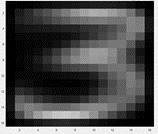
\includegraphics[width=0.55\linewidth]{mean_three.png}
%		\caption{Mean image of digit 3}
%		\label{fig:mean_three}
%	\end{subfigure}
%	\begin{subfigure}[b]{0.49\textwidth}
%		\centering
%		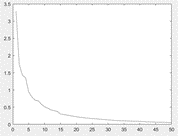
\includegraphics[width=0.6\linewidth]{50_largest_eigenvalues.png}
%		\caption{Eigenvalues}
%		\label{fig:50_largest_eigenvalues}
%	\end{subfigure}
%	\begin{subfigure}[b]{1.0\textwidth}
%		\centering
%		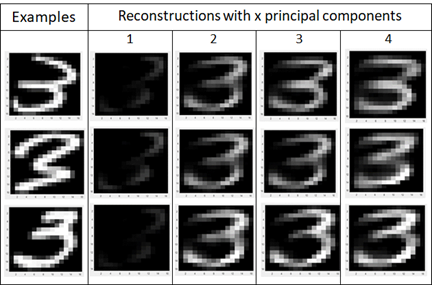
\includegraphics[width=0.4\linewidth]{reconstruction_x_principal_eigenvalues.png}
%		\caption{Increasing amount of eigenvectors}
%		\label{fig:increasing_eigenvectors}
%	\end{subfigure}		
%	\caption{Results of applying PCA on the US Postal Service database.}
%	\label{fig:Results1}
%\end{figure}


%\begin{table}
%	\centering
%	\begin{tabular}{@{}clr@{}} \toprule
%		\textbf{Attractor} & \textbf{Point} & \textbf{Stability}\\\midrule
%		Attractor $ 1 $ & $ [1;1] $ & Stable\\
%		Attractor $ 2 $ & $ [-1;-1] $ & Stable\\
%		Attractor $ 3 $ & $ [1;-1] $ & Stable\\
%		Attractor $ 4 $ & $ [-1;1] $ & Stable\\
%		Attractor $ 5 $ & $ [0;0] $ & Unstable\\
%		Attractor $ 6 $ & $ [0;1] $ & Unstable\\
%		Attractor $ 7 $ & $ [0;-1] $ & Unstable\\
%		Attractor $ 8 $ & $ [1;0] $ & Unstable\\
%		Attractor $ 9 $ & $ [-1;0] $ & Unstable\\\bottomrule
%	\end{tabular}
%	\caption{Overview of the different attractor points found in a 2D plane.}
%	\label{tab:att}
%\end{table}

\bibliographystyle{abbrv}
%\bibliography{ANN1}

\end{document}
